% Berkeley Math Tournament 2024
\section*{One Funny Lemma That Almost Caught Me Offguard}
\subsection*{Sebuah Lemma dari Berkeley Math Tournament 2024}
\textbf{Sedikit keluh kesah:} Jadi, aku dapet soal ini dari Wildan. Awalnya aku nemu caranya pake Inversi. Terus mikir dong, masa soal "selucu ini" ngga ada cara biasanya (non projective solution)? Tapi, malah nyari pake cara biasa malah lama banget ngga ketemu-temu (aku nyoba beberapa minggu lalu). Akhirnya semalem setelah nyoba sekali lagi, bisa ketemu :D

\section{Soal}
Lingkaran dalam segitiga sembarang tak sama kaki $\triangle ABC$ menyinggung sisi $\overline{BC}, \overline{AC},$ dan $\overline{AB}$ masing-masing di titik $D, E,$ dan $F$. Garis $EF$ memotong garis $BC$ di titik $P$ dan garis $AD$ di titik $Q$. Lingkaran luar segitiga $\triangle AEF$ memotong kembali garis $AP$ di titik $R \neq A$. Jika $I$ adalah titik pusat lingkaran dalam segitiga $\triangle ABC$, buktikan bahwa titik-titik $I, Q, R$ terletak pada satu garis lurus.

\begin{center}
\definecolor{rvwvcq}{rgb}{0.08235294117647059,0.396078431372549,0.7529411764705882}
\definecolor{wewdxt}{rgb}{0.43137254901960786,0.42745098039215684,0.45098039215686275}
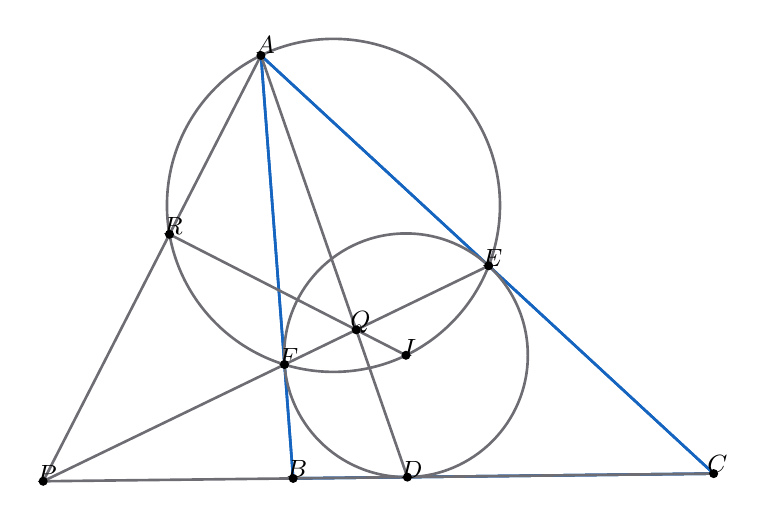
\begin{tikzpicture}[scale=1.26,line cap=round,line join=round]
  \draw[line width=0.95pt,color=rvwvcq] (0.07,0.32)--(0.39464,-3.94283)--(4.63288,-3.89433)--cycle;
  \draw[line width=0.95pt,color=rvwvcq] (0.07,0.32)--(0.39464,-3.94283);
  \draw[line width=0.95pt,color=rvwvcq] (0.39464,-3.94283)--(4.63288,-3.89433);
  \draw[line width=0.95pt,color=rvwvcq] (4.63288,-3.89433)--(0.07,0.32);
  \draw[line width=0.95pt,color=wewdxt] (0.80085,-1.19086) circle (1.67834);
  \draw[line width=0.95pt,color=wewdxt] (0.07,0.32)--(-2.12531,-3.97166);
  \draw[line width=0.95pt,color=wewdxt] (0.07,0.32)--(1.54575,-3.92966);
  \draw[line width=0.95pt,color=wewdxt] (-0.85198,-1.4824)--(1.5317,-2.70172);
  \draw[line width=0.95pt,color=wewdxt] (1.5317,-2.70172) circle (1.22802);
  \draw[line width=0.95pt,color=wewdxt] (-2.12531,-3.97166)--(4.63288,-3.89433);
  \draw[line width=0.95pt,color=wewdxt] (2.3649,-1.7996)--(-2.12531,-3.97166);
  \fill (0.07,0.32) circle (1.3pt);
  \node[font=\small] at (0.11339,0.42149) {$A$};
  \fill (0.39464,-3.94283) circle (1.3pt);
  \node[font=\small] at (0.43343,-3.84584) {$B$};
  \fill (4.63288,-3.89433) circle (1.3pt);
  \node[font=\small] at (4.67167,-3.79735) {$C$};
  \fill (1.5317,-2.70172) circle (1.3pt);
  \node[font=\small] at (1.56816,-2.62383) {$I$};
  \fill (1.54575,-3.92966) circle (1.3pt);
  \node[font=\small] at (1.58755,-3.85554) {$D$};
  \fill (2.3649,-1.7996) circle (1.3pt);
  \node[font=\small] at (2.40223,-1.72187) {$E$};
  \fill (0.30722,-2.79497) circle (1.3pt);
  \node[font=\small] at (0.34615,-2.72082) {$F$};
  \fill (-2.12531,-3.97166) circle (1.3pt);
  \node[font=\small] at (-2.08817,-3.89433) {$P$};
  \fill (1.03026,-2.44521) circle (1.3pt);
  \node[font=\small] at (1.07353,-2.37167) {$Q$};
  \fill (-0.85198,-1.4824) circle (1.3pt);
  \node[font=\small] at (-0.81767,-1.40182) {$R$};
\end{tikzpicture}
\end{center}


\newpage
\section{Solusi 1, Synthetic - Euclid Solution}
    \begin{remark*}[Motivasi]
        Karena nemu solusi 2 duluan, jadi kepikiran, emang jangan-jangan ini soal banyak yang siklisnya biar bisa di \textbf{angle chasing} atau dihajar pake \textbf{power of a point}. Terus berkali-kali konstruksi titik yang pas akhirnya nemu kalau jika dikonstruksi titik $H$, maka ada 5 segiempat siklis yang berguna untuk angle chasing di akhir :).
    \end{remark*}
    Misalkan $I$ adalah titik pusat lingkaran dalam $\triangle ABC$. Lalu, misalkan $H$ adalah perotongan $AI$ dengan $FE$ dan $G$ adalah titik di $AD$ sehingga $IG \perp AD$.

    \input{TikzLatex/31-sol1}
    
    Perhatikan bahwa $\dangle AFI = \dangle AEI = 90^\circ$ sehingga $A,F,I,E$ konsiklis dengan $AI$ sebagai diameternya. 
    Selanjutnya, karena $\dangle DGI = 90^\circ$ maka $D,G,I$ konsiklis dengan $DI$ sebagai diameternya. Di lain sisi, karena $\dangle IGA = 90^\circ = \dangle IFA$, maka $A,I,F,G$ konsiklis. 
    Lebih jauh, garis $IG$ merupakan \textit{radical axis} dari lingkaran $(AFGI)$ dan $(EGI)$.
    
    Selanjutnya, karena $DI \perp BC$ maka $(D,G,I)$ menyinggung $BC$ di $D$. Namun, karena $(DEF)$ juga menyinggung $BC$ di $D$ maka $BC$ merupakan \textit{radical axis} dari $(DEF)$ dan $(DGI)$.

    Di lain pihak, kita juga punya $EF$ merupakan \textit{radical axis} dari $(AEF)$ dan $(DEF)$.

    Perhatikan bahwa ketiga \textit{radical axis} $EF, BC, IG$ konkuren di suatu \textit{radical point}. Dari definisi di soal, karena $P$ adalah perpotongan $EF$ dan $BC$, maka didapat $P$ merupakan \textit{radical center} dari $(AEF), (DEF), (DGI)$.

    Misalkan $\Gamma$ adalah lingkaran yang melalui $A$ dan menyinggung $BC$ di $D$. Dari \textit{power of a point}, kita punya
    \begin{align*}
        PR \cdot PA = PF \cdot PE = PG \cdot PI = PD^2,
    \end{align*}
    sehingga didapat $R$ berada di $\Gamma$.

    Sekarang, jelas bahwa $EF \perp AI$ sehingga $\dangle QHI = 90^\circ = \dangle QGI$ yang menunjukkan $Q,H,I,G$ konsiklis. Oleh karena itu, dari \textit{power of a point} kita punya
    \begin{align*}
        PR \cdot PA = PG \cdot PI = PQ \cdot PH,
    \end{align*}
    sehingga didapat $A,R,Q,H$ konsiklis dengan $\dangle QRA = \dangle QHA = 90^\circ$. 
    Padahal kita juga tahu bahwa $A,R,F,I,E$ konsiklis dengan $AI$ sebagai diameternya yang langsung menyebabkan $\dangle IRA = 90^\circ$. Dari sini didapat $I,Q,R$ segaris. Terbukti.

\newpage
\section{Solusi 2, Inversi - Projective Geometry}
    Kita akan memakai konfigurasi gambar dari solusi 1.
        \begin{center}
\definecolor{rvwvcq}{rgb}{0.08235294117647059,0.396078431372549,0.7529411764705882}
\definecolor{wewdxt}{rgb}{0.43137254901960786,0.42745098039215684,0.45098039215686275}
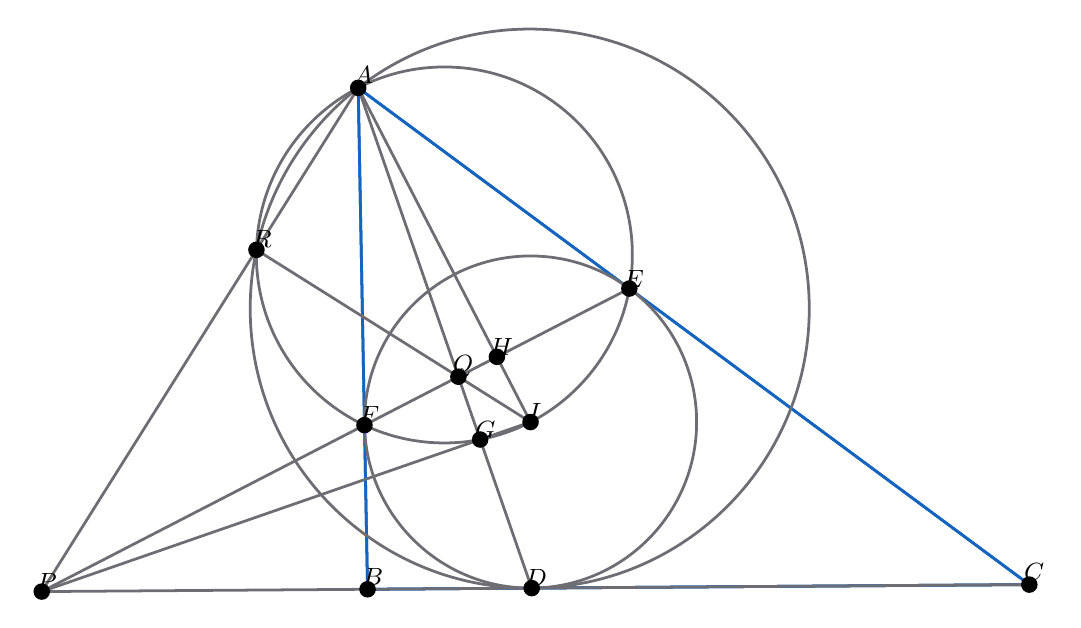
\begin{tikzpicture}[scale=2.3,line cap=round,line join=round]
  \draw[line width=1.00pt,color=rvwvcq] (-0.63636,0.37624)--(-0.58477,-2.39231)--(3.06937,-2.36652)--cycle;
  \draw[line width=1.00pt,color=rvwvcq] (-0.63636,0.37624)--(-0.58477,-2.39231);
  \draw[line width=1.00pt,color=rvwvcq] (-0.58477,-2.39231)--(3.06937,-2.36652);
  \draw[line width=1.00pt,color=rvwvcq] (3.06937,-2.36652)--(-0.63636,0.37624);
  \draw[line width=1.00pt,color=wewdxt] (-0.16058,-0.54634) circle (1.03804);
  \draw[line width=1.00pt,color=wewdxt] (-0.63636,0.37624)--(-2.3837,-2.40501);
  \draw[line width=1.00pt,color=wewdxt] (-0.63636,0.37624)--(0.32167,-2.38591);
  \draw[line width=1.00pt,color=wewdxt] (-1.19823,-0.5181)--(0.3152,-1.46892);
  \draw[line width=1.00pt,color=wewdxt] (0.3152,-1.46892)--(-2.3837,-2.40501);
  \draw[line width=1.00pt,color=wewdxt] (0.31078,-0.84247) circle (1.54348);
  \draw[line width=1.00pt,color=wewdxt] (0.3152,-1.46892) circle (0.91702);
  \draw[line width=1.00pt,color=wewdxt] (-0.63636,0.37624)--(0.3152,-1.46892);
  \draw[line width=1.00pt,color=wewdxt] (-2.3837,-2.40501)--(3.06937,-2.36652);
  \draw[line width=1.00pt,color=wewdxt] (0.86075,-0.73183)--(-2.3837,-2.40501);
  \fill (-0.63636,0.37624) circle (1.3pt);
  \node[font=\small] at (-0.60909,0.44702) {$A$};
  \fill (-0.58477,-2.39231) circle (1.3pt);
  \node[font=\small] at (-0.55451,-2.32287) {$B$};
  \fill (3.06937,-2.36652) circle (1.3pt);
  \node[font=\small] at (3.09548,-2.29558) {$C$};
  \fill (0.3152,-1.46892) circle (1.3pt);
  \node[font=\small] at (0.33923,-1.41549) {$I$};
  \fill (0.32167,-2.38591) circle (1.3pt);
  \node[font=\small] at (0.34605,-2.3297) {$D$};
  \fill (0.86075,-0.73183) circle (1.3pt);
  \node[font=\small] at (0.88502,-0.67867) {$E$};
  \fill (-0.60166,-1.486) circle (1.3pt);
  \node[font=\small] at (-0.57497,-1.42914) {$F$};
  \fill (-2.3837,-2.40501) circle (1.3pt);
  \node[font=\small] at (-2.35562,-2.35016) {$P$};
  \fill (-0.08319,-1.21863) circle (1.3pt);
  \node[font=\small] at (-0.05647,-1.16306) {$Q$};
  \fill (-1.19823,-0.5181) circle (1.3pt);
  \node[font=\small] at (-1.16852,-0.46036) {$R$};
  \fill (0.03708,-1.56538) circle (1.3pt);
  \node[font=\small] at (0.06633,-1.51101) {$G$};
  \fill (0.12955,-1.10892) circle (1.3pt);
  \node[font=\small] at (0.15502,-1.05391) {$H$};
\end{tikzpicture}
\end{center}

    Observasi inversi terhadap lingkaran $(DEF)$. 
    Karena $\triangle IFH \sim \triangle IAF$ maka $IH \cdot IA = IF^2$ dengan $IF$ adalah jari-jari lingkaran $(DEF)$, maka $EF$ dipetakan ke $(AEF)$.
    Lalu, $\triangle IGD \sim \triangle IDP$ sehingga $IG \cdot IP = ID^2$ dengan $ID$ adalah jari-jari lingkaran $(DEF)$, maka $G$ dipetakan ke $P$.

    Perhatikan bahwa $AD$ adalah \textit{polar} dari \textit{pole} $P$ karena $IG \perp AD$.
    Misalkan $Q$ dipetakan ke $R'$ yang berada di $(AEF)$. Ingat bahwa $AI$ adalah diameter $(AEF)$ maka $IR' \perp AR'$. 
    Lalu, $AR'$ adalah \textit{polar} dari \textit{pole} $Q$. 
    Namun, perlu diingat bahwa karena $Q$ berada di \textit{polar} dari $P$, maka dari \textit{La Hire's theorem} didapat $P$ berada di \textit{polar} dari $Q$. Dari sini didapat $P$ berada di $AR'$.

    Dikarenakan $R$ dan $R'$ berada di $(AEF)$ serta $A,R,R',P$ segaris, maka didapat $R=R'$. Terbukti bahwa $I,Q,R'=R$ segaris.
